\chapter{引言}
\subsection{背景}

Kobayashi--Hitchin 对应这一概念，源于 M. S. Narasimhan 与 C. S. Seshadri \cite{Na-Se} 的一项极具洞见的发现：在紧黎曼曲面上，基本群的不可约酉表示与其上次数为零的稳定全纯向量丛之间存在对应关系。随后在 S. K. Donaldson \cite{Do1,Do2}、S. Kobayashi \cite{Ko1,Ko2}、L\"ubke \cite{Lu}、Hitchin \cite{Hc}、Uhlenbeck 与 Yau \cite{Uh-Yau} 等人的持续推动下，这一理论发展成其现代形式：在紧 Kähler 流形 \(X\) 上实现如下“三位一体”：
\begin{center}
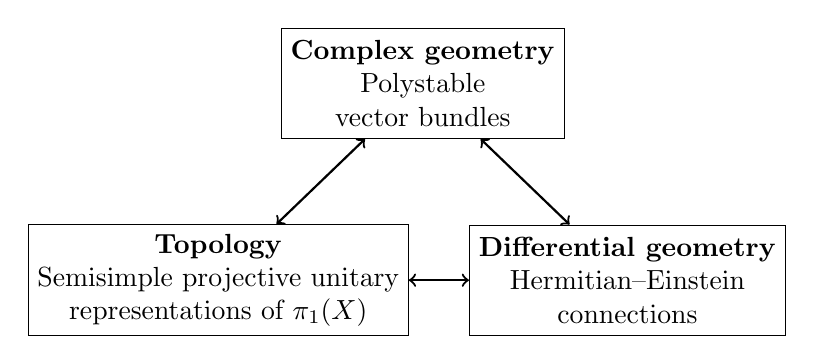
\begin{tikzpicture}[
    every node/.style={draw, rectangle, align=center, minimum width=3.5cm, minimum height=1.4cm},
    arrow/.style={<->, thick}
]

% Define the triangle nodes using polar coordinates
\node (A) at (90:1cm) {\textbf{Complex geometry}\\Polystable\\vector bundles};
\node (B) at (210:3cm) {\textbf{Topology}\\Semisimple projective unitary\\representations of $\pi_1(X)$};
\node (C) at (330:3cm) {\textbf{Differential geometry}\\Hermitian--Einstein\\connections};

% Draw arrows (bidirectional)
\draw[arrow] (A) -- (B);
\draw[arrow] (B) -- (C);
\draw[arrow] (C) -- (A);

\end{tikzpicture}
\end{center}
当我们研究 \(X\) 上稳定向量丛的模空间时，这一对应使模空间能够从不同视角交织出丰富的几何结构。

另一个推广方向是考虑拟射影情形中的对应问题。V. Mehta 与 C. S. Seshadri \cite{Me-Se} 在研究带穿孔黎曼曲面 \(X^\circ\) 的基本群酉表示时开创了这一方向，这可看作是对 Narasimhan 与 Seshadri \cite{Na-Se} 工作的推广。在他们的论文中，建立了 \(X^\circ\) 的基本群酉表示与其紧化 \(X\) 上稳定抛物丛概念之间的对应。受其启发，抛物向量丛的概念逐渐推广到更高维情形。为说明起见，我们先考虑最简单的情况。

设 \((X,\omega)\) 是一个紧 Kähler 流形，\(D\) 是一个光滑不可约除子。一个抛物丛是一个二元组
\[
F_*=(F,\mathcal F),
\]
其中 \(F\to X\) 是底层全纯向量丛，而 \(\mathcal F\) 是沿除子给定的抛物结构。抛物结构 \(\mathcal F\) 是 \(F|_D\) 上一列递降的全纯子丛过滤：
\[
F|_D = F_0 \supset F_1 \supset F_2 \supset \cdots \supset F_\ell \supset 0,
\]
并为各 \(F_i\) 赋权
\[
0\le a_i < a_{i+1} <1.
\]
我们使用下标“\(*\)”来强调抛物结构；若省略“\(*\)”而只写 \(F\)，则表示抛物丛的底层丛。与普通向量丛情形一样，抛物丛也有相应的抛物 Chern 特征、次数、关于 \(\omega\) 的斜率稳定性等概念。关于抛物丛，还有其他刻画方式，可参见例如 \cite{Bw,Iy-Si,Mo2}。更一般地，也可以定义一般除子上的抛物层。它最初由 M. Maruyama 与 K. Yokogawa \cite{Ma-Yo} 为研究模问题而引入。但在本文中，我们遵循 T. Mochizuki 在 \cite[Chapter 3]{Mo1} 中给出的定义。细节见第 2 节。

自 1990 年代以来，抛物丛吸引了大量关注。更重要也更迷人的是研究带有 Higgs 场且沿除子具有对数奇性的抛物丛，因为这会导向拟射影光滑簇上的非阿贝尔 Hodge 对应，该方向由 C. T. Simpson \cite{Si1} 开创。这个主题试图将上文“三位一体”中的对象替换为：拟射影簇上的半单局部系统、调和丛以及 Chern 类平凡的稳定抛物 Higgs 丛。J. Jost 与 K. Zuo \cite{Jo-Ka} 建立了前两类对象之间的桥梁，而 T. Mochizuki \cite{Mo3} 建立了后两类对象之间的桥梁。O. Biquard \cite{Bi} 处理了底空间为带光滑除子的 Kähler 流形的情形。若底空间为带简单正规交叉除子的 Kähler 流形，该问题仍然是开放的。如今，这一主题依然活跃，研究者试图把背景推广到带某些奇性的空间上的层，例如 Klt、Dlt 簇。当没有 Higgs 场时，这个问题也曾在不同背景下被例如 \cite{Li,Li-Nasimhan,St-Wr} 考虑。

特别地，第二作者在 \cite{Li} 中证明：对于带简单正规交叉除子 \(D\) 的紧 Kähler 流形 \((X,\omega)\)，一个抛物丛 \(F_*\) 关于 \(\omega\) 稳定，当且仅当在 \(F|_{X\setminus D}\) 上存在关于某个锥型 Kähler 度量 \(\omega_\delta\)（即在 \(D\) 附近有温和奇性的度量）的 Hermitian--Einstein 度量 \(H_\delta\)，并且 \(H_\delta\) 与抛物结构相容。作为结果，作者得到了抛物版本的 Bogomolov--Gieseker 不等式。

\subsection{目的}

值得注意的是，尽管第二作者所用的锥型度量 \(\omega_\delta\) 在流的意义下与 \(\omega\) 属于同一个上同调类，但只能得到关于 \(\omega_\delta\) 而不是 \(\omega\) 的 Hermitian--Einstein 度量，这并不十分理想。本文的目的，是将先前结果推广到半稳定抛物层的情形，并同时解决这一问题。下面简要描述我们的主要结果。

设 \(F_*\) 是与 \((X,\omega,D)\) 相关的一个秩为 \(r\) 的饱和自反抛物层。记 \(\ch_k(\cdot)\) 为抛物层的第 \(k\) 个 Chern 特征算子。与通常一样，定义抛物层 \(F_*\) 的次数为
\[
\deg_\omega(F_*):=\ch_1(F_*)\cdot \frac{[\omega]^{n-1}}{(n-1)!},
\]
其斜率定义为
\[
\mu_\omega(F_*):=\frac{\deg_\omega(F_*)}{\rank(F_*)}.
\]
我们称 \(F_*\) 关于 Kähler 度量 \(\omega\) 是 \(\mu_\omega\)-稳定（或简称 \(\omega\)-稳定）的（分别地，半稳定的），如果对任意真抛物子层 \(S_*\) 都有
\[
\mu_\omega(S_*)<(\text{分别地 } \le)\,\mu_\omega(F_*).
\]

从第 2 节可知，\(F_*\) 在一个余维至少为 3 的解析子集 \(W\) 之外是局部阿贝尔的抛物丛。记
\[
X^\circ:=X-W,\qquad \mathcal F_*:=F_*|_{X^\circ}.
\]
在本文其余部分中，我们有时将 \(F\) 简称为 \(F\) 的正则部分，而将 \(F|_{X^\circ\setminus D}\) 称作 \(F_*\) 的正则部分。

\begin{definition}
称 \(F|_{X^\circ\setminus D}\) 上的一个 Hermitian 度量 \(H\) 与抛物层 \(F_*\)（或其抛物结构）相容，如果满足下列条件：
\begin{enumerate}[label=\arabic*.]
\item
\[
\frac{\sqrt{-1}}{2\pi}\tr(F_H)
\]
表示 \(\ch_1(F_*)\)，其中 \(F_H\) 是 Chern 曲率张量。
\item 对任意真抛物子层 \(S_*\subset F_*\)，设 \(H|_{S_*}\) 为 \(S_*\) 正则部分上的诱导度量，则在流的意义下有
\[
\ch_1(S_*)\le \frac{\sqrt{-1}}{2\pi}\tr(F_{H|_{S_*}}).
\]
\end{enumerate}
如果进一步满足
\begin{itemize}
\item \(F_H\in L^2(H,\omega)\)；
\item \(\Lambda F_H\in L^\infty(H)\)，其中 \(\Lambda F_H\) 表示相对于 \(\omega\) 的收缩，
\end{itemize}
则称 \(H\) 是\textbf{可容许的}（admissible）。
\end{definition}

\begin{remark}
当 \(F_*\) 是抛物丛时，条件 2 中的不等式可以加强为等式。但在层的情形中，这是我们所能期望的最好结果。
\end{remark}

自反层上的可容许度量这一概念最早由 S. Bando 与 Y. Siu 在 \cite{B-S} 中引入，他们研究了自反层的 Kobayashi--Hitchin 问题。

\begin{definition}
设 \(F\) 是 Kähler 流形 \((X,\omega)\) 上的一个向量丛。若一个 Hermitian 度量 \(H\) 满足
\[
\sqrt{-1}\Lambda_\omega F_H-\lambda\cdot \id_F=0
\]
在整个 \(X\) 上成立，其中 \(\lambda\) 是实常数，\(\Lambda_\omega\) 是 Lefschetz 算子的伴随，则称 \(H\) 为 \textbf{Hermitian--Einstein}（H-E）度量。
\end{definition}

\begin{definition}
设 \(F\) 是 Kähler 流形 \((X,\omega)\) 上的一个向量丛。若一族由 \(t\in[0,\infty)\) 参数化的 Hermitian 度量 \(H(t)\) 满足
\[
\lim_{t\to\infty}\bigl\|\sqrt{-1}\Lambda_\omega F_{H(t)}-\lambda\cdot \id_F\bigr\|_{L^\infty(X,H(t))}=0,
\]
则称其为\textbf{近似 Hermitian--Einstein}（approximate H-E）度量族。
\end{definition}

我们得到如下定理：

\begin{theorem}[定理 6.14]
设 \(F_*\) 是 \((X,\omega,D)\) 上的一个饱和自反抛物层。则 \(F_*\) 是 \(\mu_\omega\)-多稳定的，当且仅当在 \(F|_{X^\circ\setminus D}\) 上存在一个关于 \(\omega\) 的、与 \(F_*\) 相容的可容许 H-E 度量。
\end{theorem}

\begin{theorem}[定理 6.15]
设 \(F_*\) 是 \((X,\omega,D)\) 上的一个饱和自反抛物层。则 \(F_*\) 是 \(\mu_\omega\)-半稳定的，当且仅当在 \(F|_{X^\circ\setminus D}\) 上存在一族关于 \(\omega\) 的、与 \(F_*\) 相容的可容许近似 H-E 度量。
\end{theorem}

作为推论，我们得到抛物版本的 Bogomolov--Gieseker 不等式。记
\[
\Delta(F_*):=\frac{\ch_1(F_*)^2}{2\rank(F_*)}-\ch_2(F_*)
\]
为 Bogomolov--Gieseker 判别式。

\begin{corollary}[推论 6.16]
若 \(F_*\) 关于 \(\omega\) 是 \(\mu_\omega\)-半稳定的，则
\[
\Delta(F_*)\cdot [\omega]^{n-2}\ge 0.
\]
此外，若 \(F_*\) 是多稳定的，则等号成立当且仅当 \(F|_{X\setminus D}\) 是一个向量丛，且它带有一个与抛物结构相容的射影平坦 H-E 联络。
\end{corollary}

为层建立 Bogomolov--Gieseker 不等式使我们在应用中有更大的灵活性。作为结果，我们还证明了：

\begin{theorem}[定理 7.1]
设 \(F_*\) 是紧 Kähler 流形 \((X,\omega)\) 上的一个饱和自反抛物层，并且它关于一个 nef 且 big 的类 \([\eta]\) 是半稳定的。那么关于 \([\eta]\) 的 Bogomolov--Gieseker 不等式成立，即
\[
\Delta(F_*)\cdot [\eta]^{n-2}\ge 0.
\]
\end{theorem}

\subsection{文章结构}

\begin{itemize}
\item \S2：我们引入一个以抛物层为对象的阿贝尔范畴。粗略地说，一个抛物层 \(F_*\) 是一族仅在除子 \(D\) 上退化的层过滤。我们讨论态射、Chern 特征、次数、稳定性条件等概念。我们还证明，一个饱和自反抛物层 \(F_*\) 在余维至少为 3 的解析集之外是抛物丛。

\item \S3：我们通过沿 \(W\) 上方的光滑中心连续爆破来解消 \(F_*\) 的奇性。总之，我们得到一个修改 \(\pi:\widetilde X\to X\)。设 \(E\) 为例外除子。为简化记号，我们对由 \(\pi\) 拉回的对象仍使用原记号。于是，在 \(\widetilde X\) 上，\(F\) 可以嵌入一个局部自由层 \(\mathcal E\) 中，且在 \(E\) 外 \(\mathcal E\) 与 \(F\) 同构。再经进一步爆破后，\(\mathcal E\) 将从 \(F_*\) 继承抛物结构。记该抛物丛为 \(\mathcal E_*\)。

\item \S4：为了利用 Hermitian--Yang--Mills 流来变形 \(F_*\) 正则部分上的度量，我们首先在 \(\widetilde X-D\) 上构造一族由 \(\pi^*\omega\) 导出的锥型 Kähler 度量 \(\omega^\varepsilon_\delta\)。特别地，这族度量满足一个具有统一常数的 Sobolev 型不等式。相应地，我们在 \(\mathcal E_*\) 上构造一个奇异 Hermitian 度量 \(H^\varepsilon\)，它在 \(D\) 的严格变换上退化为零。然后我们证明，\(H^\varepsilon\) 的曲率张量能像普通向量丛那样给出 \(\mathcal E_*\) 的第一与第二 Chern 特征。我们相信所构造的这个抛物度量实际上给出所有抛物 Chern 特征。由于 \(\widetilde X\) 与 \(X\) 在 \(W\) 外同构，它也诱导出 \(F_*\) 正则部分上的一个度量。正如预期，\(H^\varepsilon\) 的曲率张量将给出 \(F_*\) 的第一与第二 Chern 特征。

\item \S5：我们回顾向量丛相对于丛上的 Hermitian 度量与底流形上的 Kähler 形式的解析稳定性概念。更重要的是，我们证明 Hermitian 全纯向量丛 \((F|_{X^\circ\setminus D},H^\varepsilon)\) 的解析稳定性等价于抛物层 \(F_*\) 的稳定性。

\item \S6：我们分析相对于锥型 Kähler 度量 \(\omega^\varepsilon_\delta\) 及初始度量 \(H^\varepsilon\) 的一族 Hermitian--Yang--Mills (H-Y-M) 流，在丛 \(\mathcal E|_{\widetilde X-D}\) 上：
\[
\begin{cases}
H^{-1}\dfrac{dH}{dt}
=
-2\bigl(\sqrt{-1}\Lambda_{\omega^\varepsilon_\delta}F_H-\lambda^\varepsilon_\delta\cdot \id_F\bigr),\\[0.7em]
\det(H)=\det(H^\varepsilon),\\
H(0)=H^\varepsilon.
\end{cases}
\]
我们证明，当 \(\varepsilon,\delta\to 0\) 时，这族流收敛到定义在 \(F_*\) 正则部分上的流
\[
\begin{cases}
H^{-1}\dfrac{dH}{dt}
=
-2\bigl(\sqrt{-1}\Lambda_\omega F_H-\lambda\cdot \id_F\bigr),\\[0.7em]
\det(H)=\det(H^\varepsilon),\\
H(0)=H^\varepsilon,
\end{cases}
\]
其中
\[
\lambda:=\frac{2\pi\cdot \mu_\omega(F_*)}{\operatorname{Vol}(X,\omega)}.
\]
然后我们证明，在稳定（分别地，半稳定）条件下，该流将收敛到 \(F|_{X^\circ\setminus D}\) 上一个与 \(F_*\) 相容的可容许 H-E 度量（分别地，一族可容许近似 H-E 度量）。我们也将证明其逆命题，其中 H-E 度量的可容许性是关键。

\item \S7：作为应用，我们利用 Jordan--H\"older 过滤证明：关于 big 且 nef 类的半稳定抛物层满足 Bogomolov--Gieseker 型不等式。
\end{itemize}